% answers.tex —— 2009 年·普通高等学校招生考试·浙江卷·文科 · 参考答案与详细解析片段
% 由 tools/generate_projects.py 依来源总账自 2009/2009_数学真题_浙江文_试题.md + 2009/2009_数学真题_浙江文_解析正文.md + 2009/2009_数学真题_浙江文_答案要点.md 生成，勿手改（改源 MD 后重跑）


\begin{gktip}
固定候选 PDF 仅含题面，无答案、解析和评分标准，原页亦未标分值；以下为非官方编者独立推导，官方答案字段为空。题面文字层按栏混排严重，只作定位；分数、根号、上下标与六幅图均以 600 dpi 原页复核。原页第 15 题第二张表的表头误印为「高峰」，按题文与表题取低谷电价 0.288、0.318、0.388。
\end{gktip}

\begin{answer}
\gksolhead{1}{}

\textbf{题目}：

设 $U=\mathbf R$，$A=\{x\mid x>0\}$，$B=\{x\mid x>1\}$，则 $A\cap\complement_U B=$（　）

（A）$\{x\mid 0\leqslant x<1\}$

（B）$\{x\mid 0<x\leqslant 1\}$

（C）$\{x\mid x<0\}$

（D）$\{x\mid x>1\}$

\Needspace{4\baselineskip}
\textbf{解析}

$B=\{x\mid x>1\}$，故 $\complement_U B=\{x\mid x\leqslant1\}$。

$A$ 与它取交集：$x$ 须同时满足 $x>0$ 与 $x\leqslant1$，即 $0<x\leqslant1$。

端点检验：$x=1$ 在 $\complement_U B$ 中且 $1>0$，故 $1$ 可取（右端为闭）；$x=0$ 不在 $A$ 中，故 $0$ 不可取（左端为开）。选项 (B) 与此一致。

\gkanswer{答案：B。}

\end{answer}
\begin{answer}
\gksolhead{2}{}

\textbf{题目}：

“$x>0$”是“$x\neq0$”的（　）

（A）充分而不必要条件

（B）必要而不充分条件

（C）充分必要条件

（D）既不充分也不必要条件

\Needspace{4\baselineskip}
\textbf{解析}

充分性：若 $x>0$，则必有 $x\neq0$。

必要性：取 $x=-1$，它满足 $x\neq0$，但不满足 $x>0$，故不能由 $x\neq0$ 推出 $x>0$。

因此“$x>0$”是“$x\neq0$”的充分而不必要条件。

\gkanswer{答案：A。}

\end{answer}
\begin{answer}
\gksolhead{3}{}

\textbf{题目}：

设 $z=1+\mathrm i$（$\mathrm i$ 是虚数单位），则 $\dfrac2z+z^2=$（　）

（A）$1+\mathrm i$

（B）$-1+\mathrm i$

（C）$1-\mathrm i$

（D）$-1-\mathrm i$

\Needspace{4\baselineskip}
\textbf{解析}

$\dfrac2z=\dfrac{2}{1+\mathrm i}=\dfrac{2(1-\mathrm i)}{(1+\mathrm i)(1-\mathrm i)}=\dfrac{2(1-\mathrm i)}2=1-\mathrm i$。

$z^2=(1+\mathrm i)^2=1+2\mathrm i+\mathrm i^2=2\mathrm i$。

相加得 $\dfrac2z+z^2=1-\mathrm i+2\mathrm i=1+\mathrm i$。

\gkanswer{答案：A。}

\end{answer}
\begin{answer}
\gksolhead{4}{}

\textbf{题目}：

设 $\alpha$，$\beta$ 是两个不同的平面，$l$ 是一条直线，以下命题正确的是（　）

（A）若 $l\perp\alpha$，$\alpha\perp\beta$，则 $l\subset\beta$

（B）若 $l\parallel\alpha$，$\alpha\parallel\beta$，则 $l\subset\beta$

（C）若 $l\perp\alpha$，$\alpha\parallel\beta$，则 $l\perp\beta$

（D）若 $l\parallel\alpha$，$\alpha\perp\beta$，则 $l\perp\beta$

\Needspace{4\baselineskip}
\textbf{解析}

逐项判断：

\begin{itemize}
\item （A）取 $\alpha:z=0$，$\beta:x=0$，直线 $l:\{(1,0,t)\mid t\in\mathbf R\}$。$l$ 的方向向量 $(0,0,1)$ 垂直于 $\alpha$，$\alpha\perp\beta$，但 $l$ 不在 $\beta$ 内，故（A）错；
\item （B）取 $\alpha:z=0$，$\beta:z=1$，$l:\{(t,0,\tfrac12)\mid t\in\mathbf R\}$。$l\parallel\alpha$，$\alpha\parallel\beta$，但 $l$ 不在 $\beta$ 内，故（B）错；
\item （C）若 $l\perp\alpha$，则 $l$ 的方向向量是 $\alpha$ 的法向量；$\alpha\parallel\beta$ 说明 $\alpha$ 与 $\beta$ 有相同的法向量方向，故 $l\perp\beta$。正确；
\item （D）仍取（A）中的 $\alpha$，$\beta$ 与 $l:\{(t,0,0)\mid t\in\mathbf R\}$，则 $l\parallel\alpha$，$\alpha\perp\beta$，但 $l$ 在 $\alpha$ 内，不垂直于 $\beta$，故（D）错。
\end{itemize}

\gkanswer{答案：C。}

\end{answer}
\begin{answer}
\gksolhead{5}{}

\textbf{题目}：

已知向量 $\boldsymbol a=(1,2)$，$\boldsymbol b=(2,-3)$．若向量 $\boldsymbol c$ 满足 $(\boldsymbol c+\boldsymbol a)\parallel\boldsymbol b$，$\boldsymbol c\perp(\boldsymbol a+\boldsymbol b)$，则 $\boldsymbol c=$（　）

（A）$\left(\frac79,\frac73\right)$

（B）$\left(-\frac73,-\frac79\right)$

（C）$\left(\frac73,\frac79\right)$

（D）$\left(-\frac79,-\frac73\right)$

\Needspace{4\baselineskip}
\textbf{解析}

设 $\boldsymbol c=(x,y)$。由 $\boldsymbol a=(1,2)$，$\boldsymbol b=(2,-3)$ 得 $\boldsymbol a+\boldsymbol b=(3,-1)$。

\Needspace{5\baselineskip}
$\boldsymbol c\perp(\boldsymbol a+\boldsymbol b)$ 给出

\nopagebreak[4]
\[3x-y=0,\qquad y=3x.\]

\Needspace{5\baselineskip}
又 $\boldsymbol c+\boldsymbol a=(x+1,3x+2)$，它与 $\boldsymbol b=(2,-3)$ 平行，故

\nopagebreak[4]
\[-3(x+1)-2(3x+2)=0.\]

即 $-9x-7=0$，$x=-\dfrac79$，从而 $y=-\dfrac73$。所求为 $\left(-\dfrac79,-\dfrac73\right)$，对应（D）。

\gkanswer{答案：D。}

\end{answer}
\begin{answer}
\gksolhead{6}{}

\textbf{题目}：

已知椭圆 $\dfrac{x^2}{a^2}+\dfrac{y^2}{b^2}=1$（$a>b>0$）的左焦点为 $F$，右顶点为 $A$，点 $B$ 在椭圆上，且 $BF\perp x$ 轴，直线 $AB$ 交 $y$ 轴于点 $P$．若 $\overrightarrow{AP}=2\overrightarrow{PB}$，则椭圆的离心率是（　）

（A）$\frac{\sqrt3}{2}$

（B）$\frac{\sqrt2}{2}$

（C）$\frac13$

（D）$\frac12$

\Needspace{4\baselineskip}
\textbf{解析}

设焦距参数为 $c=\sqrt{a^2-b^2}$，左焦点 $F(-c,0)$，右顶点 $A(a,0)$。

\Needspace{5\baselineskip}
$BF\perp x$ 轴，故 $B$ 的横坐标为 $-c$。代入椭圆方程，

\nopagebreak[4]
\[\frac{c^2}{a^2}+\frac{y^2}{b^2}=1
\quad\Longrightarrow\quad
\frac{y^2}{b^2}=1-\frac{c^2}{a^2}=\frac{b^2}{a^2},\]

故 $B\left(-c,\dfrac{b^2}{a}\right)$（取上方，取下方不影响横坐标）。

\Needspace{5\baselineskip}
设 $P(0,p)$。由 $\overrightarrow{AP}=2\overrightarrow{PB}$ 得

\nopagebreak[4]
\[P-A=2(B-P)\quad\Longrightarrow\quad P=\frac{A+2B}{3}.\]

\Needspace{5\baselineskip}
比较横坐标：

\nopagebreak[4]
\[0=\frac{a+2(-c)}3\quad\Longrightarrow\quad a=2c.\]

故离心率 $e=\dfrac ca=\dfrac12$，对应（D）。纵坐标条件只用来确定 $p$，不影响 $e$。

\gkanswer{答案：D。}

\end{answer}
\begin{answer}
\gksolhead{7}{}

\textbf{题目}：

某程序框图如图所示，该程序运行后输出的 $k$ 的值是（　）

（A）$4$

（B）$5$

（C）$6$

（D）$7$
\nopagebreak[4]
\begin{center}% 2009 年浙江卷文科第 7 题：程序框图。
%   开始 → k=0 → S=0 → 判断 S<100?
%   是 → S=S+2^S → k=k+1 → 回到判断；否 → 输出 k → 结束。
% 来源 PDF：普通高考/2009/2009浙江文.pdf，SHA-256 8e609d19459cb4234a4d6dd9db5be5c8cc9af2169c00d4337b3988089cfb0709。
% 原页：第 1 页（A3 三栏）第 1 栏下部，书页码 567。
% 重绘依据：原页方框内为 S=S+2^S（指数为 S，非 k，已按 600 dpi 逐字复核），
%   判断框菱形，输出用平行四边形，「是」向下、「否」向右。
\begin{tikzpicture}[scale=1.0, semithick,
  every node/.style={inner sep=2pt, font=\small},
  box/.style={draw, minimum width=2.35cm, minimum height=0.62cm, align=center},
  term/.style={draw, rounded corners=6pt, minimum width=1.9cm,
    minimum height=0.60cm, align=center},
  para/.style={draw, trapezium, trapezium left angle=70,
    trapezium right angle=110, minimum width=2.0cm, minimum height=0.62cm,
    align=center},
  dec/.style={draw, diamond, aspect=2.6, minimum width=2.5cm,
    minimum height=1.05cm, align=center, inner sep=1pt},
  arr/.style={->, >=stealth}]

  \node[term] (start) at (0,8.3) {开始};
  \node[box] (k0) at (0,7.30) {$k=0$};
  \node[box] (s0) at (0,6.25) {$S=0$};
  \node[dec] (test) at (0,4.90) {$S<100?$};
  \node[box] (add) at (0,3.45) {$S=S+2^{S}$};
  \node[box] (inc) at (0,2.35) {$k=k+1$};
  \node[para] (out) at (4.6,4.90) {输出 $k$};
  \node[term] (end) at (4.6,3.85) {结束};

  \draw[arr] (start) -- (k0);
  \draw[arr] (k0) -- (s0);
  \draw[arr] (s0) -- (test);
  \draw[arr] (test) -- node[left] {是} (add);
  \draw[arr] (add) -- (inc);
  % 回到判断
  \draw[arr] (inc.west) -- ++(-1.55,0) |- (test.west);
  % 否分支
  \draw[arr] (test.east) -- node[above] {否} (out.west);
  \draw[arr] (out) -- (end);
\end{tikzpicture}
\end{center}
\nopagebreak[4]
\Needspace{4\baselineskip}
\textbf{解析}

初值 $k=0$，$S=0$。判断框为 $S<100$，“是”向下执行 $S=S+2^S$ 与 $k=k+1$ 后返回判断，“否”向右输出 $k$。逐步计算：

\begin{itemize}
\item $S=0<100$：$S=0+2^0=1$，$k=1$；
\item $S=1<100$：$S=1+2^1=3$，$k=2$；
\item $S=3<100$：$S=3+2^3=11$，$k=3$；
\item $S=11<100$：$S=11+2^{11}=2059$，$k=4$；
\item $S=2059\geqslant100$：退出循环，输出 $k=4$。
\end{itemize}

注：指数为 $S$ 而不是 $k$。若误读为 $S=S+2^k$，$S$ 的序列将是 $1,3,7,15,31,63,127$，会输出 $7$；原页方框内指数确为 $S$（600 dpi 逐字复核）。

\gkanswer{答案：A。}

\end{answer}
\begin{answer}
\gksolhead{8}{}

\textbf{题目}：

若函数 $f(x)=x^2+\dfrac ax$（$a\in\mathbf R$），则下列结论正确的是（　）

（A）$\forall a\in\mathbf R$，$f(x)$ 在 $(0,+\infty)$ 上是增函数

（B）$\forall a\in\mathbf R$，$f(x)$ 在 $(0,+\infty)$ 上是减函数

（C）$\exists a\in\mathbf R$，$f(x)$ 是偶函数

（D）$\exists a\in\mathbf R$，$f(x)$ 是奇函数

\Needspace{4\baselineskip}
\textbf{解析}

\Needspace{5\baselineskip}
$f(x)=x^2+\dfrac ax$，定义域为 $x\neq0$。求导：

\nopagebreak[4]
\[f'(x)=2x-\frac{a}{x^2}=\frac{2x^3-a}{x^2}.\]

在 $(0,+\infty)$ 上，$f'$ 的符号由 $2x^3-a$ 决定。

\begin{itemize}
\item 若 $a\leqslant0$，则 $2x^3-a>0$，$f$ 在 $(0,+\infty)$ 上递增；
\item 若 $a>0$，则 $f'$ 在 $x=\sqrt[3]{\dfrac a2}$ 处由负变正，$f$ 先减后增。
\end{itemize}

所以（A）（B）都不可能对一切 $a$ 成立。

再看奇偶性。取 $a=0$，则 $f(x)=x^2$（$x\neq0$），定义域关于原点对称，且 $f(-x)=(-x)^2=x^2=f(x)$，故 $f$ 为偶函数，（C）正确。

\Needspace{5\baselineskip}
若 $f$ 为奇函数，则对一切 $x\neq0$ 有

\nopagebreak[4]
\[x^2+\frac ax=-x^2-\frac ax\quad\Longrightarrow\quad 2x^2=0,\]

不可能，故（D）不对。

\gkanswer{答案：C。}

\end{answer}
\begin{answer}
\gksolhead{9}{}

\textbf{题目}：

已知三角形的三边长分别为 $3$，$4$，$5$，则它的边与半径为 $1$ 的圆的公共点个数最多为（　）

（A）$3$

（B）$4$

（C）$5$

（D）$6$

\Needspace{4\baselineskip}
\textbf{解析}

\Needspace{5\baselineskip}
三边 $3$，$4$，$5$ 满足 $3^2+4^2=5^2$，是直角三角形，其内切圆半径

\nopagebreak[4]
\[r=\frac{3+4-5}{2}=1.\]

半径为 $1$ 的圆若要与三条边所在直线都相交于两点，圆心到三条直线的距离必须都小于 $1$。但三角形内到三边距离都不超过 $1$ 的点只有内心，此时三个距离恰为 $1$，圆与三边相切，只有 $3$ 个公共点。因此不可能三条边各交出两点。

于是至多两条边各交于两点，第三条边至多相切（$1$ 点）或不相交，公共点至多 $4$ 个。

\Needspace{5\baselineskip}
$4$ 个可以实现：以直角顶点为原点、两直角边为坐标轴，取圆心 $(0.9,0.9)$，圆与两直角边各交于两点，且交点在边内；圆心到斜边 $3x+4y=12$ 的距离为

\nopagebreak[4]
\[\frac{|2.7+3.6-12|}{5}=1.14>1,\]

不与斜边相交。故最多为 $4$，对应（B）。

\gkanswer{答案：B。}

\end{answer}
\begin{answer}
\gksolhead{10}{}

\textbf{题目}：

已知 $a$ 是实数，则函数 $f(x)=1+a\sin ax$ 的图象不可能是（　）
\nopagebreak[4]
\begin{center}% 2009 年浙江卷文科第 10 题：函数 f(x)=1+a\sin(ax) 的四个候选图象（A）—（D）。
% 来源 PDF：普通高考/2009/2009浙江文.pdf，SHA-256 8e609d19459cb4234a4d6dd9db5be5c8cc9af2169c00d4337b3988089cfb0709。
% 原页：第 1 页第 2 栏上部，书页码 567。
% 重绘依据：四幅小图均以虚线标出 y=1、y=2 与 x=\pi、x=2\pi。
%   （A）最大值约 1.8、最小值约 0.2（即 |a|<1）且周期约 2.4\pi；
%   （B）最大值约 2.2、最小值约 -0.2（|a|>1），周期约 1.7\pi；
%   （C）恒为 y=1（a=0）；
%   （D）最大值约 2.2、最小值约 -0.2，但相邻最大值与最小值相距约 1.1\pi（> \pi），
%       与 |a|>1 时相距 \pi/|a|<\pi 矛盾，故按原页原样重绘其形状。
\begin{tikzpicture}[semithick, every node/.style={inner sep=1.2pt, font=\small}]

  % ================= 面板 (A) =================
  \begin{scope}[shift={(0,0)}]
    \draw[-{Stealth}] (0,0) -- (4.75,0) node[right] {$x$};
    \draw[-{Stealth}] (0,-0.55) -- (0,2.55) node[above] {$y$};
    \node[below left=1pt] at (0,0) {$O$};
    \draw[dashed] (0,0.95) -- (4.55,0.95);
    \draw[dashed] (0,1.90) -- (4.55,1.90);
    \draw[dashed] (1.99,0) -- (1.99,2.45);
    \draw[dashed] (3.98,0) -- (3.98,2.45);
    \node[below] at (1.99,0) {$\pi$};
    \node[below] at (3.98,0) {$2\pi$};
    \node[left] at (0,0.95) {$1$};
    \node[left] at (0,1.90) {$2$};
    \draw[thick] plot[domain=0:7.0,samples=140]
      ({0.6335*\x}, {0.95*(1+0.8*sin(0.8*\x r))});
    \node at (0.55,-0.95) {(A)};
  \end{scope}

  % ================= 面板 (B) =================
  \begin{scope}[shift={(6.0,0)}]
    \draw[-{Stealth}] (0,0) -- (4.75,0) node[right] {$x$};
    \draw[-{Stealth}] (0,-0.55) -- (0,2.55) node[above] {$y$};
    \node[below left=1pt] at (0,0) {$O$};
    \draw[dashed] (0,0.95) -- (4.55,0.95);
    \draw[dashed] (0,1.90) -- (4.55,1.90);
    \draw[dashed] (1.99,0) -- (1.99,2.45);
    \draw[dashed] (3.98,0) -- (3.98,2.45);
    \node[below] at (1.99,0) {$\pi$};
    \node[below] at (3.98,0) {$2\pi$};
    \node[left] at (0,0.95) {$1$};
    \node[left] at (0,1.90) {$2$};
    \draw[thick] plot[domain=0:6.35,samples=140]
      ({0.6335*\x}, {0.95*(1+1.2*sin(1.2*\x r))});
    \node at (0.55,-0.95) {(B)};
  \end{scope}

  % ================= 面板 (C) =================
  \begin{scope}[shift={(0,-4.75)}]
    \draw[-{Stealth}] (0,0) -- (4.75,0) node[right] {$x$};
    \draw[-{Stealth}] (0,-0.55) -- (0,2.55) node[above] {$y$};
    \node[below left=1pt] at (0,0) {$O$};
    \draw[dashed] (1.99,0) -- (1.99,2.45);
    \draw[dashed] (3.98,0) -- (3.98,2.45);
    \node[below] at (1.99,0) {$\pi$};
    \node[below] at (3.98,0) {$2\pi$};
    \node[left] at (0,0.95) {$1$};
    \node[left] at (0,1.90) {$2$};
    \draw[thick] (0,0.95) -- (4.55,0.95);
    \node at (0.55,-0.95) {(C)};
  \end{scope}

  % ================= 面板 (D) =================
  \begin{scope}[shift={(6.0,-4.75)}]
    \draw[-{Stealth}] (0,0) -- (4.75,0) node[right] {$x$};
    \draw[-{Stealth}] (0,-0.55) -- (0,2.55) node[above] {$y$};
    \node[below left=1pt] at (0,0) {$O$};
    \draw[dashed] (0,0.95) -- (4.55,0.95);
    \draw[dashed] (0,1.90) -- (4.55,1.90);
    \draw[dashed] (1.99,0) -- (1.99,2.45);
    \draw[dashed] (3.98,0) -- (3.98,2.45);
    \node[below] at (1.99,0) {$\pi$};
    \node[below] at (3.98,0) {$2\pi$};
    \node[left] at (0,0.95) {$1$};
    \node[left] at (0,1.90) {$2$};
    % 按原页：峰在 \pi/2 之右约 0.55\pi、谷在约 1.65\pi，两峰谷相距超过 \pi
    \draw[thick] plot[smooth] coordinates {
      (0,0.95) (0.30,1.20) (0.60,1.55) (0.85,1.85) (1.09,2.09)
      (1.35,2.03) (1.65,1.75) (1.95,1.35) (2.20,0.95) (2.50,0.52)
      (2.85,0.17) (3.10,0.00) (3.31,-0.16) (3.60,-0.12) (3.85,0.08)
      (3.98,0.24) (4.30,0.75) (4.58,1.33)
    };
    \node at (0.55,-0.95) {(D)};
  \end{scope}
\end{tikzpicture}
\end{center}
\nopagebreak[4]
\Needspace{4\baselineskip}
\textbf{解析}

记 $A=|a|$。由 $f(x)=1+a\sin(ax)$ 得：最大值为 $1+A$，最小值为 $1-A$，相邻的最大值与最小值横坐标相差半个周期 $\dfrac{\pi}{A}$；又 $f(0)=1$，$f'(0)=a^2\geqslant0$。

逐图核对：

\begin{itemize}
\item （A）：最大值约 $1.8$、最小值约 $0.2$，都介于 $0$ 与 $2$ 之间，故 $A<1$，周期 $\dfrac{2\pi}{A}>2\pi$，一个周期内只出现一个峰、一个谷，且峰在 $\dfrac\pi2$ 之右、谷在 $2\pi$ 之前，与 $A\approx0.8$ 的图形一致；
\item （B）：最大值约 $2.2$、最小值约 $-0.2$，故 $A>1$，峰谷相距 $\dfrac{\pi}{A}<\pi$；图中峰在 $0.4\pi$ 附近、谷在 $1.25\pi$ 附近，相距约 $0.85\pi$，与 $A\approx1.2$ 一致；
\item （C）：图象为直线 $y=1$，即 $a=0$，可能；
\item （D）：最大值约 $2.2$、最小值约 $-0.2$，同样要求 $A>1$；但 $A>1$ 时最大值应在 $x=\dfrac{\pi}{2A}<\dfrac\pi2$ 处，且与相邻最小值相距 $\dfrac{\pi}{A}<\pi$。图中最大值在 $\dfrac\pi2$ 之右（约 $0.55\pi$），最小值在 $1.6\pi$ 之后，两者相距超过 $\pi$，矛盾。故（D）不可能是 $f(x)=1+a\sin(ax)$ 的图象。
\end{itemize}

\gkanswer{答案：D。}

\end{answer}
\begin{answer}
\gksolhead{11}{}

\textbf{题目}：

设等比数列 $\{a_n\}$ 的公比 $q=\dfrac12$，前 $n$ 项和为 $S_n$，则 $\dfrac{S_4}{a_4}=$\gkblank{}．

\Needspace{4\baselineskip}
\textbf{解析}

\Needspace{5\baselineskip}
$S_4=\dfrac{a_1(1-q^4)}{1-q}$，$a_4=a_1q^3$。当 $q=\dfrac12$ 时，

\nopagebreak[4]
\[\frac{S_4}{a_4}
=\frac{1-q^4}{(1-q)q^3}
=\frac{1+q+q^2+q^3}{q^3}
=\frac{1}{q^3}+\frac1{q^2}+\frac1q+1.\]

\Needspace{5\baselineskip}
代入 $q=\dfrac12$：

\nopagebreak[4]
\[\frac{S_4}{a_4}=8+4+2+1=15.\]

\gkanswer{答案：$15$。}

\end{answer}
\begin{answer}
\gksolhead{12}{}

\textbf{题目}：

若某几何体的三视图（单位：cm）如图所示，则此几何体的体积是\gkblank{}$\mathrm{cm^3}$．
\nopagebreak[4]
\begin{center}% 2009 年浙江卷文科第 12 题：三视图（正视图、侧视图、俯视图）。
% 来源 PDF：普通高考/2009/2009浙江文.pdf，SHA-256 8e609d19459cb4234a4d6dd9db5be5c8cc9af2169c00d4337b3988089cfb0709。
% 原页：第 1 页第 2 栏中部，书页码 567。单位 cm。
% 重绘依据：正视图为 T 形，上横条宽 3（三段各 1）、高 1，竖柱宽 1、高 3；
%   侧视图为 3×4 矩形，距顶 1 处有一条横线；俯视图为 3×3 正方形，两条竖直虚线
%   为竖柱两侧棱的投影。按标注尺寸等比重绘（原页图线条未严格等比）。
\begin{tikzpicture}[semithick, every node/.style={inner sep=1.5pt, font=\small}]

  % ---------- 正视图 ----------
  \draw (0,4) -- (3,4) -- (3,3) -- (2,3) -- (2,0) -- (1,0) -- (1,3) -- (0,3) -- cycle;
  \foreach \a/\c in {0/0.5, 1/1.5, 2/2.5} {
    \draw[<->] (\a,4.28) -- (\a+1,4.28);
    \node[above] at (\c,4.28) {$1$};
  }
  \draw[<->] (3.30,3) -- (3.30,4);
  \node[right] at (3.30,3.5) {$1$};
  \draw[<->] (3.30,0) -- (3.30,3);
  \node[right] at (3.30,1.5) {$3$};
  \node at (1.5,-0.62) {正视图};

  % ---------- 侧视图 ----------
  \draw (4.90,4) -- (7.90,4) -- (7.90,0) -- (4.90,0) -- cycle;
  \draw (4.90,3) -- (7.90,3);
  \draw[<->] (4.90,4.28) -- (7.90,4.28);
  \node[above] at (6.40,4.28) {$3$};
  \node at (6.40,-0.62) {侧视图};

  % ---------- 俯视图 ----------
  \draw (0,-2) -- (3,-2) -- (3,-5) -- (0,-5) -- cycle;
  \draw[dashed] (1,-2) -- (1,-5);
  \draw[dashed] (2,-2) -- (2,-5);
  \draw[<->] (3.30,-2) -- (3.30,-5);
  \node[right] at (3.30,-3.5) {$3$};
  \node at (1.5,-5.62) {俯视图};
\end{tikzpicture}
\end{center}
\nopagebreak[4]
\Needspace{4\baselineskip}
\textbf{解析}

正视图为 T 形：上横条宽 $3$（三段各 $1$）、高 $1$，竖柱宽 $1$、高 $3$。侧视图为 $3\times4$ 矩形，距顶 $1$ 处有一条横线，说明上横条的深度为 $3$。俯视图为 $3\times3$ 正方形，两条竖直虚线是竖柱两侧棱的投影。

\Needspace{5\baselineskip}
因此几何体是上横条 $3\times3\times1$ 与竖柱 $1\times3\times3$ 的组合，体积为

\nopagebreak[4]
\[V=3\times3\times1+1\times3\times3=9+9=18\ (\mathrm{cm^3}).\]

\gkanswer{答案：$18$。}

\end{answer}
\begin{answer}
\gksolhead{13}{}

\textbf{题目}：

若实数 $x$，$y$ 满足不等式组 $\begin{cases}x+y\geqslant2,\\2x-y\leqslant4,\\x-y\geqslant0,\end{cases}$ 则 $2x+3y$ 的最小值是\gkblank{}．

\Needspace{4\baselineskip}
\textbf{解析}

三条边界直线为 $x+y=2$，$2x-y=4$，$x-y=0$。两两求交点：

\begin{itemize}
\item $x+y=2$ 与 $x-y=0$：$(1,1)$；
\item $x+y=2$ 与 $2x-y=4$：$(2,0)$；
\item $2x-y=4$ 与 $x-y=0$：$(4,4)$。
\end{itemize}

\Needspace{5\baselineskip}
可行域是以这三点为顶点的三角形。目标函数 $z=2x+3y$ 在三点的值分别为

\nopagebreak[4]
\[z(1,1)=5,\qquad z(2,0)=4,\qquad z(4,4)=20.\]

线性函数在三角形上的最小值必在顶点取得，故最小值为 $4$（在 $(2,0)$ 处）。

\gkanswer{答案：$4$。}

\end{answer}
\begin{answer}
\gksolhead{14}{}

\textbf{题目}：

某个容量为 $100$ 的样本的频率分布直方图如下，则在区间 $[4,5)$ 上的数据的频数为\gkblank{}．
\nopagebreak[4]
\begin{center}% 2009 年浙江卷文科第 14 题：频率分布直方图。
% 来源 PDF：普通高考/2009/2009浙江文.pdf，SHA-256 8e609d19459cb4234a4d6dd9db5be5c8cc9af2169c00d4337b3988089cfb0709。
% 原页：第 1 页第 3 栏上部，书页码 567。
% 重绘依据：横轴 0—6，0 与 1 之间为省略断轴；纵轴为「频率/组距」。
%   各组矩形高：[1,2)=0.05，[2,3)=0.10，[3,4)=0.40，[4,5)=0.30，[5,6)=0.15。
%   虚线标出 0.05、0.10、0.15、0.40 四条水平参考线。
\begin{tikzpicture}[x=1.25cm, y=9.0cm, semithick,
  every node/.style={inner sep=1.5pt, font=\small}]

  % 坐标轴
  \draw[-{Stealth}] (-0.15,0) -- (6.55,0) node[right] {数据};
  \draw[-{Stealth}] (0,-0.025) -- (0,0.505);
  \node[align=center] at (0.58,0.468) {频率\\[-2pt]组距};

  % 水平虚线
  \foreach \h in {0.05,0.10,0.15,0.40} {
    \draw[dashed] (0,\h) -- (6.15,\h);
  }

  % 各组矩形
  \draw (1,0) rectangle (2,0.05);
  \draw (2,0) rectangle (3,0.10);
  \draw (3,0) rectangle (4,0.40);
  \draw (4,0) rectangle (5,0.30);
  \draw (5,0) rectangle (6,0.15);

  % 断轴符号（0 与 1 之间）
  \draw (0.22,0) -- (0.30,0.018) -- (0.38,0) -- (0.46,0.018) -- (0.54,0);

  % 刻度与标签
  \foreach \x in {1,2,3,4,5,6} {
    \draw (\x,0) -- (\x,-0.006);
    \node[below] at (\x,-0.008) {$\x$};
  }
  \node[below left=1pt] at (0,0) {$O$};
  \node[left] at (0,0.05) {$0.05$};
  \node[left] at (0,0.10) {$0.10$};
  \node[left] at (0,0.15) {$0.15$};
  \node[left] at (0,0.40) {$0.40$};
\end{tikzpicture}
\end{center}
\nopagebreak[4]
\Needspace{4\baselineskip}
\textbf{解析}

\Needspace{5\baselineskip}
直方图的纵轴是“频率/组距”，组距为 $1$，故每一组的小矩形面积等于该组频率。图中 $[4,5)$ 一组的高为 $0.30$，频率为

\nopagebreak[4]
\[0.30\times1=0.30.\]

\Needspace{5\baselineskip}
样本容量为 $100$，所以该组频数为

\nopagebreak[4]
\[0.30\times100=30.\]

核对：各组高依次为 $[1,2)$ 的 $0.05$、$[2,3)$ 的 $0.10$、$[3,4)$ 的 $0.40$、$[5,6)$ 的 $0.15$，合计 $0.05+0.10+0.40+0.30+0.15=1.00$，与总频率为 $1$ 一致。

\gkanswer{答案：$30$。}

\end{answer}
\begin{answer}
\gksolhead{15}{}

\textbf{题目}：

某地区居民生活用电分为高峰和低谷两个时间段进行分时计价．该地区的电网销售电价表如下：

高峰时间段用电价格表

\begin{center}
\begin{tabular}{ll}
\toprule
高峰月用电量（单位：千瓦时） & 高峰电价（单位：元/千瓦时） \\
\midrule
50 及以下的部分 & 0.568 \\
超过 50 至 200 的部分 & 0.598 \\
超过 200 的部分 & 0.668 \\
\bottomrule
\end{tabular}
\end{center}

低谷时间段用电价格表

\begin{center}
\begin{tabular}{ll}
\toprule
高峰月用电量（单位：千瓦时） & 高峰电价（单位：元/千瓦时） \\
\midrule
50 及以下的部分 & 0.288 \\
超过 50 至 200 的部分 & 0.318 \\
超过 200 的部分 & 0.388 \\
\bottomrule
\end{tabular}
\end{center}

若某家庭 5 月份的高峰时间段用电量为 $200$ 千瓦时，低谷时间段用电量为 $100$ 千瓦时，则按这种计费方式该家庭本月应付的电费为\gkblank{}元．（用数字作答）

\Needspace{4\baselineskip}
\textbf{解析}

原页第二张表的表头误印为“高峰月用电量”“高峰电价”，但表题明写“低谷时间段用电价格表”，题文也说“低谷时间段用电量”，故按表题取该表所列低谷电价 $0.288$，$0.318$，$0.388$。

\Needspace{5\baselineskip}
高峰用电 $200$ 千瓦时，分两档：

\nopagebreak[4]
\[50\times0.568+(200-50)\times0.598=28.4+89.7=118.1.\]

\Needspace{5\baselineskip}
低谷用电 $100$ 千瓦时，分两档：

\nopagebreak[4]
\[50\times0.288+(100-50)\times0.318=14.4+15.9=30.3.\]

\Needspace{5\baselineskip}
合计

\nopagebreak[4]
\[118.1+30.3=148.4\ (\text{\text{元}}).\]

\gkanswer{答案：$148.4$。}

\end{answer}
\begin{answer}
\gksolhead{16}{}

\textbf{题目}：

设等差数列 $\{a_n\}$ 的前 $n$ 项和为 $S_n$，则 $S_4$，$S_8-S_4$，$S_{12}-S_8$，$S_{16}-S_{12}$ 成等差数列．类比以上结论有：设等比数列 $\{b_n\}$ 的前 $n$ 项积为 $T_n$，则 $T_4$，\gkblank{}，\gkblank{}，$\dfrac{T_{16}}{T_{12}}$ 成等比数列．

\Needspace{4\baselineskip}
\textbf{解析}

\Needspace{5\baselineskip}
设等比数列 $\{b_n\}$ 的公比为 $q$，则

\nopagebreak[4]
\[T_n=b_1^nq^{1+2+\cdots+(n-1)}=b_1^nq^{\frac{n(n-1)}2}.\]

\Needspace{5\baselineskip}
于是

\nopagebreak[4]
\[T_4=b_1^4q^6,\qquad
\frac{T_8}{T_4}=b_1^4q^{22},\qquad
\frac{T_{12}}{T_8}=b_1^4q^{38},\qquad
\frac{T_{16}}{T_{12}}=b_1^4q^{54}.\]

\Needspace{5\baselineskip}
相邻两项之比：

\nopagebreak[4]
\[\frac{T_8/T_4}{T_4}=q^{16},\qquad
\frac{T_{12}/T_8}{T_8/T_4}=q^{16},\qquad
\frac{T_{16}/T_{12}}{T_{12}/T_8}=q^{16}.\]

比值相同，故 $T_4$，$\dfrac{T_8}{T_4}$，$\dfrac{T_{12}}{T_8}$，$\dfrac{T_{16}}{T_{12}}$ 成等比数列。

\gkanswer{答案：$\dfrac{T_8}{T_4}$，$\dfrac{T_{12}}{T_8}$。}

\end{answer}
\begin{answer}
\gksolhead{17}{}

\textbf{题目}：

有 $20$ 张卡片，每张卡片上分别标有两个连续的自然数 $k$，$k+1$，其中 $k=0$，$1$，$2$，$\cdots$，$19$．从这 $20$ 张卡片中任取一张，记事件“该卡片上两个数的各位数字之和（例如：若取到标有 $9$，$10$ 的卡片，则卡片上两个数的各位数字之和为 $9+1+0=10$）不小于 $14$”为 $A$，则 $P(A)=$\gkblank{}．

\Needspace{4\baselineskip}
\textbf{解析}

逐张计算卡片 $\{k,k+1\}$ 上两个数的各位数字之和 $g(k)$：

\begin{center}
\begingroup\setlength{\tabcolsep}{4pt}
\begin{tabular}{lllllllllll}
\toprule
$k$ & $0$ & $1$ & $2$ & $3$ & $4$ & $5$ & $6$ & $7$ & $8$ & $9$ \\
\midrule
$g(k)$ & $1$ & $3$ & $5$ & $7$ & $9$ & $11$ & $13$ & $15$ & $17$ & $10$ \\
\bottomrule
\end{tabular}
\endgroup
\end{center}

\begin{center}
\begingroup\setlength{\tabcolsep}{4pt}
\begin{tabular}{lllllllllll}
\toprule
$k$ & $10$ & $11$ & $12$ & $13$ & $14$ & $15$ & $16$ & $17$ & $18$ & $19$ \\
\midrule
$g(k)$ & $3$ & $5$ & $7$ & $9$ & $11$ & $13$ & $15$ & $17$ & $19$ & $12$ \\
\bottomrule
\end{tabular}
\endgroup
\end{center}

\Needspace{5\baselineskip}
不小于 $14$ 的有 $k=7,8,16,17,18$，共 $5$ 张。故

\nopagebreak[4]
\[P(A)=\frac5{20}=\frac14.\]

\gkanswer{答案：$\dfrac14$。}

\end{answer}
\begin{answer}
\gksolhead{18}{}

\textbf{题目}：

在 $\triangle ABC$ 中，角 $A$，$B$，$C$ 所对的边分别为 $a$，$b$，$c$，且满足 $\cos\dfrac A2=\dfrac{2\sqrt5}{5}$，$\overrightarrow{AB}\cdot\overrightarrow{AC}=3$．

（1）求 $\triangle ABC$ 的面积；

（2）若 $c=1$，求 $a$ 的值．

\Needspace{4\baselineskip}
\textbf{解析}

\Needspace{5\baselineskip}
（1）由 $\cos\dfrac A2=\dfrac{2\sqrt5}{5}$ 得

\nopagebreak[4]
\[\cos A=2\cos^2\frac A2-1=2\times\frac45-1=\frac35.\]

\Needspace{5\baselineskip}
因为 $A$ 为三角形内角，$\sin A>0$，故

\nopagebreak[4]
\[\sin A=\sqrt{1-\frac{9}{25}}=\frac45.\]

\Needspace{5\baselineskip}
又

\nopagebreak[4]
\[\overrightarrow{AB}\cdot\overrightarrow{AC}
=|\overrightarrow{AB}||\overrightarrow{AC}|\cos A
=bc\cdot\frac35=3,\]

\Needspace{5\baselineskip}
故 $bc=5$。面积

\nopagebreak[4]
\[S=\frac12bc\sin A=\frac12\times5\times\frac45=2.\]

\Needspace{5\baselineskip}
（2）由 $c=1$ 得 $b=5$。由余弦定理，

\nopagebreak[4]
\[a^2=b^2+c^2-2bc\cos A
=25+1-2\times5\times1\times\frac35
=26-6=20,\]

故 $a=2\sqrt5$。

检验：$b=5$，$c=1$，$a=2\sqrt5$ 满足 $a^2=20=b^2+c^2-2bc\cos A$，且三角形不等式 $1+2\sqrt5>5$ 成立。

\gkanswer{答案：（1）$2$；（2）$a=2\sqrt5$。}

\end{answer}
\begin{answer}
\gksolhead{19}{}

\textbf{题目}：

如图，$DC\perp$ 平面 $ABC$，$EB\parallel DC$，$AC=BC=EB=2DC=2$，$\angle ACB=120^\circ$，$P$，$Q$ 分别为 $AE$，$AB$ 的中点．

（1）证明：$PQ\parallel$ 平面 $ACD$；

（2）求 $AD$ 与平面 $ABE$ 所成角的正弦值．
\nopagebreak[4]
\begin{center}% 2009 年浙江卷文科第 19 题：DC⊥平面 ABC，EB∥DC，AC=BC=EB=2DC=2，
% ∠ACB=120°，P、Q 分别为 AE、AB 的中点。
% 来源 PDF：普通高考/2009/2009浙江文.pdf，SHA-256 8e609d19459cb4234a4d6dd9db5be5c8cc9af2169c00d4337b3988089cfb0709。
% 原页：第 2 页第 1 栏上部，书页码 568。
% 重绘依据：按斜二测投影重绘；D 在 C 正上方、E 在 B 正上方，DC 与 EB 均画成
%   竖直；C 在底面 ABC 内，故 CA、CB、CD 为虚线，其余可见棱为实线。
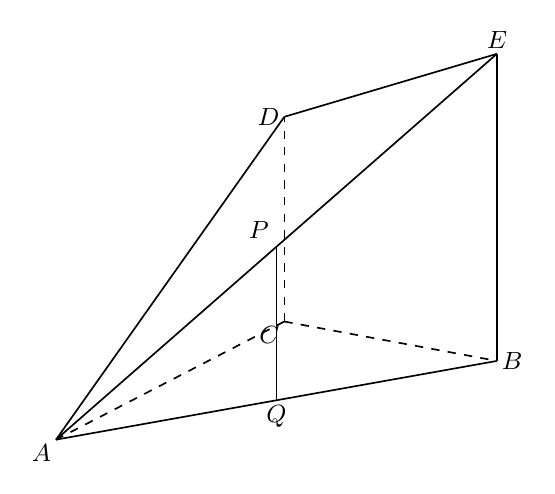
\begin{tikzpicture}[semithick, every node/.style={inner sep=1.5pt, font=\small}]
  \coordinate (A) at (0,0);
  \coordinate (B) at (5.6,1.0);
  \coordinate (C) at (2.9,1.5);
  \coordinate (D) at (2.9,4.1);
  \coordinate (E) at (5.6,4.9);
  \coordinate (P) at (2.8,2.45);
  \coordinate (Q) at (2.8,0.5);

  % 可见棱
  \draw (A) -- (B);
  \draw (A) -- (D);
  \draw (A) -- (E);
  \draw (D) -- (E);
  \draw (E) -- (B);
  \draw (P) -- (Q);

  % 被遮挡的棱
  \draw[dashed] (C) -- (A);
  \draw[dashed] (C) -- (B);
  \draw[dashed] (C) -- (D);

  % 标签
  \node[below left] at (A) {$A$};
  \node[right] at (B) {$B$};
  \node[below left] at (C) {$C$};
  \node[left] at (D) {$D$};
  \node[above] at (E) {$E$};
  \node[above left=1pt] at (P) {$P$};
  \node[below] at (Q) {$Q$};
\end{tikzpicture}
\end{center}
\nopagebreak[4]
\Needspace{4\baselineskip}
\textbf{解析}

\Needspace{5\baselineskip}
取 $C$ 为原点，平面 $ABC$ 为 $z=0$ 平面。由 $AC=BC=2$，$\angle ACB=120^\circ$，可令

\nopagebreak[4]
\[A(2,0,0),\qquad B(-1,\sqrt3,0).\]

$DC\perp$ 平面 $ABC$，$DC=1$，故 $D(0,0,1)$。$EB\parallel DC$，$EB=2$，故 $E(-1,\sqrt3,2)$。

\Needspace{5\baselineskip}
（1）$P$，$Q$ 分别为 $AE$，$AB$ 的中点，故

\nopagebreak[4]
\[P\left(\frac12,\frac{\sqrt3}2,1\right),\qquad
Q\left(\frac12,\frac{\sqrt3}2,0\right).\]

\Needspace{5\baselineskip}
于是

\nopagebreak[4]
\[\overrightarrow{PQ}=(0,0,-1)\parallel\overrightarrow{DC}=(0,0,-1).\]

平面 $ACD$ 由 $C(0,0,0)$，$A(2,0,0)$，$D(0,0,1)$ 确定，其方程为 $y=0$。$Q$ 的 $y$ 坐标为 $\dfrac{\sqrt3}2\neq0$，故 $Q\notin$ 平面 $ACD$，$PQ$ 不在该平面内。由线面平行判定定理，$PQ\parallel$ 平面 $ACD$。

\Needspace{5\baselineskip}
（2）$\overrightarrow{AD}=(-2,0,1)$。平面 $ABE$ 内两向量

\nopagebreak[4]
\[\overrightarrow{AB}=(-3,\sqrt3,0),\qquad
\overrightarrow{AE}=(-3,\sqrt3,2).\]

\Needspace{5\baselineskip}
法向量

\nopagebreak[4]
\[\boldsymbol n=\overrightarrow{AB}\times\overrightarrow{AE}
=(2\sqrt3,6,0).\]

\Needspace{5\baselineskip}
设 $AD$ 与平面 $ABE$ 所成角为 $\theta$，则

\nopagebreak[4]
\[\sin\theta
=\frac{|\overrightarrow{AD}\cdot\boldsymbol n|}
{|\overrightarrow{AD}||\boldsymbol n|}
=\frac{|(-2)\cdot2\sqrt3|}{\sqrt5\cdot\sqrt{12}}
=\frac{2\sqrt3}{2\sqrt{15}}
=\frac{\sqrt5}{5}.\]

\gkanswer{答案：（1）证明见解析；（2）$\dfrac{\sqrt5}{5}$。}

\end{answer}
\begin{answer}
\gksolhead{20}{}

\textbf{题目}：

设 $S_n$ 为数列 $\{a_n\}$ 的前 $n$ 项和，$S_n=kn^2+n$，$n\in\mathbf N^*$，其中 $k$ 是常数．

（1）求 $a_1$ 及 $a_n$；

（2）若对于任意的 $m\in\mathbf N^*$，$a_m$，$a_{2m}$，$a_{4m}$ 成等比数列，求 $k$ 的值．

\Needspace{4\baselineskip}
\textbf{解析}

\Needspace{5\baselineskip}
（1）$a_1=S_1=k+1$。当 $n\geqslant2$ 时，

\nopagebreak[4]
\[a_n=S_n-S_{n-1}
=k[n^2-(n-1)^2]+1
=k(2n-1)+1
=2kn+1-k.\]

\Needspace{5\baselineskip}
当 $n=1$ 时，$2k+1-k=k+1=a_1$，故通项对一切 $n\in\mathbf N^*$ 成立：

\nopagebreak[4]
\[a_1=k+1,\qquad a_n=2kn+1-k.\]

\Needspace{5\baselineskip}
（2）由（1），

\nopagebreak[4]
\[a_m=2km+1-k,\quad
a_{2m}=4km+1-k,\quad
a_{4m}=8km+1-k.\]

\Needspace{5\baselineskip}
三者成等比数列，须

\nopagebreak[4]
\[a_{2m}^2=a_ma_{4m}.\]

\Needspace{5\baselineskip}
即

\nopagebreak[4]
\[(4km+1-k)^2=(2km+1-k)(8km+1-k).\]

\Needspace{5\baselineskip}
展开：

\nopagebreak[4]
\[16k^2m^2+8km(1-k)+(1-k)^2
=16k^2m^2+10km(1-k)+(1-k)^2.\]

\Needspace{5\baselineskip}
消去相同项得

\nopagebreak[4]
\[2km(1-k)=0.\]

对任意 $m\in\mathbf N^*$ 成立，故 $k=0$ 或 $k=1$。

检验：$k=0$ 时 $a_n=1$，三数 $1,1,1$ 成等比数列（公比 $1$）；$k=1$ 时 $a_n=2n$，三数 $2m,4m,8m$ 成等比数列（公比 $2$）。两者均满足条件。

\gkanswer{答案：（1）$a_1=k+1$，$a_n=2kn+1-k$；（2）$k=0$ 或 $k=1$。}

\end{answer}
\begin{answer}
\gksolhead{21}{}

\textbf{题目}：

已知函数 $f(x)=x^3+(1-a)x^2-a(a+2)x+b$（$a$，$b\in\mathbf R$）．

（1）若函数 $f(x)$ 的图象过原点，且在原点处的切线斜率是 $-3$，求 $a$，$b$ 的值；

（2）若函数 $f(x)$ 在区间 $(-1,1)$ 上不单调，求 $a$ 的取值范围．

\Needspace{4\baselineskip}
\textbf{解析}

\Needspace{5\baselineskip}
（1）图象过原点，故

\nopagebreak[4]
\[f(0)=b=0.\]

\Needspace{5\baselineskip}
求导：

\nopagebreak[4]
\[f'(x)=3x^2+2(1-a)x-a(a+2).\]

\Needspace{5\baselineskip}
原点处切线斜率为

\nopagebreak[4]
\[f'(0)=-a(a+2)=-3,\]

\Needspace{5\baselineskip}
即

\nopagebreak[4]
\[a^2+2a-3=0\quad\Longrightarrow\quad(a-1)(a+3)=0,\]

故 $a=1$ 或 $a=-3$。于是 $(a,b)=(1,0)$ 或 $(-3,0)$。

\Needspace{5\baselineskip}
（2）由

\nopagebreak[4]
\[f'(x)=3x^2+2(1-a)x-a(a+2)\]

\Needspace{5\baselineskip}
分解因式：

\nopagebreak[4]
\[f'(x)=3\left(x-a\right)\left(x+\frac{a+2}{3}\right).\]

\Needspace{5\baselineskip}
两个零点为

\nopagebreak[4]
\[x_1=a,\qquad x_2=-\frac{a+2}{3}.\]

$f$ 在 $(-1,1)$ 上不单调，等价于 $f'$ 在 $(-1,1)$ 内有\textbf{变号}零点，即至少一个零点落在 $(-1,1)$ 内，且两个零点不重合。

\begin{itemize}
\item 由 $-1<a<1$，得 $a\in(-1,1)$；
\item 由 $-1<-\dfrac{a+2}{3}<1$，即 $-3<-(a+2)<3$，亦即 $-5<a<1$。
\end{itemize}

\Needspace{5\baselineskip}
两者取并集得 $-5<a<1$。还需剔除两零点重合的情形：

\nopagebreak[4]
\[a=-\frac{a+2}{3}\iff 3a=-a-2\iff a=-\frac12 .\]

\Needspace{5\baselineskip}
此时

\nopagebreak[4]
\[f'(x)=3\left(x+\frac12\right)^2\geqslant0,\]

$f$ 在 $(-1,1)$ 上（事实上在整个 $\mathbf R$ 上）单调递增，导数只在孤立点为零而不变号，故 $a=-\dfrac12$ 不合题意。

端点检验：

\begin{itemize}
\item $a=-5$ 时，零点为 $-5$ 与 $1$；在 $(-1,1)$ 内 $f'(x)=3(x+5)(x-1)<0$，$f$ 单调递减，不含；
\item $a=1$ 时，零点为 $1$ 与 $-1$；在 $(-1,1)$ 内 $f'(x)=3(x-1)(x+1)<0$，$f$ 单调递减，不含；
\item $a=-1$ 时，零点为 $-1$ 与 $-\dfrac13$，后者在 $(-1,1)$ 内，$f$ 不单调，包含。
\end{itemize}

故取值范围为 $\left(-5,-\dfrac12\right)\cup\left(-\dfrac12,1\right)$。

\gkanswer{答案：（1）$(a,b)=(1,0)$ 或 $(-3,0)$；（2）$-5<a<1$ 且 $a\neq-\dfrac12$，即 $(-5,-\dfrac12)\cup(-\dfrac12,1)$。}

\end{answer}
\begin{answer}
\gksolhead{22}{}

\textbf{题目}：

已知抛物线 $C:x^2=2py$（$p>0$）上一点 $A(m,4)$ 到其焦点的距离为 $\dfrac{17}{4}$．

（1）求 $p$ 与 $m$ 的值；

（2）设抛物线 $C$ 上一点 $P$ 的横坐标为 $t$（$t>0$），过 $P$ 的直线交 $C$ 于另一点 $Q$，交 $x$ 轴于点 $M$，过点 $Q$ 作 $PQ$ 的垂线交 $C$ 于另一点 $N$．若 $MN$ 是 $C$ 的切线，求 $t$ 的最小值．
\nopagebreak[4]
\begin{center}% 2009 年浙江卷文科第 22 题：抛物线 C: x^2=2py 与切线、垂线构图。
% 来源 PDF：普通高考/2009/2009浙江文.pdf，SHA-256 8e609d19459cb4234a4d6dd9db5be5c8cc9af2169c00d4337b3988089cfb0709。
% 原页：第 2 页第 3 栏中部，书页码 568。
% 重绘依据：由 (1) 得 2p=1，故 C: y=x^2。按题意图原样取一组满足 MN 为切线的
%   位置（t=2/3 时的临界图）：P(2/3,4/9)，Q(-1,1)，M(2,0)，N(4,16)；
%   x 方向缩放 0.8、y 方向缩放 0.28，仅作示意，不按等比例。
\begin{tikzpicture}[semithick, every node/.style={inner sep=1.5pt, font=\small},
  x=0.8cm, y=0.28cm]
  % 坐标轴
  \draw[-{Stealth}] (-1.55,0) -- (4.25,0) node[right] {$x$};
  \draw[-{Stealth}] (0,-1.0) -- (0,5.65) node[above] {$y$};
  \node[below left=1pt] at (0,0) {$O$};

  % 抛物线 y=x^2
  \draw[thick] plot[domain=-1.42:4.28,samples=160] (\x,{\x*\x});

  % 割线 QP，延长交 x 轴于 M 并稍过 M
  \draw (-1,1) -- (2.55,-0.1833);
  % Q 到 N 的垂线（斜率为 3）
  \draw (-1,1) -- (4.28,16.84);
  % 切线 MN（斜率为 8）
  \draw (1.75,-2) -- (4.18,17.44);

  % 点
  \fill (-1,1) circle (1.7pt) node[left=5pt] {$Q$};
  \fill (0.6667,0.4444) circle (1.7pt) node[below=4pt] {$P$};
  \fill (2,0) circle (1.7pt) node[below right] {$M$};
  \fill (4,16) circle (1.7pt) node[above left=8pt] {$N$};
\end{tikzpicture}
\end{center}
\nopagebreak[4]
\Needspace{4\baselineskip}
\textbf{解析}

\Needspace{5\baselineskip}
（1）抛物线 $x^2=2py$ 的焦点为 $F\left(0,\dfrac p2\right)$，准线为 $y=-\dfrac p2$。由抛物线定义，$A(m,4)$ 到焦点的距离等于它到准线的距离：

\nopagebreak[4]
\[4+\frac p2=\frac{17}{4}\quad\Longrightarrow\quad\frac p2=\frac14\quad\Longrightarrow\quad p=\frac12.\]

\Needspace{5\baselineskip}
又 $A$ 在抛物线上，

\nopagebreak[4]
\[m^2=2p\cdot4=8p=4,\]

故 $m=\pm2$。

\Needspace{5\baselineskip}
（2）此时 $C:y=x^2$。设 $P(t,t^2)$（$t>0$），过 $P$ 的直线斜率为 $k$，与 $C$ 的另一交点为 $Q(s,s^2)$。由

\nopagebreak[4]
\[x^2-t^2=k(x-t)\quad\Longrightarrow\quad(x-t)(x+t-k)=0,\]

\Needspace{5\baselineskip}
得 $s=k-t$，即 $k=s+t$。直线方程为

\nopagebreak[4]
\[y-t^2=(s+t)(x-t).\]

\Needspace{5\baselineskip}
令 $y=0$，得 $M$ 的横坐标

\nopagebreak[4]
\[x_M=t-\frac{t^2}{s+t}=\frac{ts}{s+t}.\]

\Needspace{5\baselineskip}
过 $Q$ 作 $PQ$ 的垂线，其斜率为 $-\dfrac1{s+t}$。与 $C$ 的另一个交点 $N(n,n^2)$ 满足

\nopagebreak[4]
\[x^2-s^2=-\frac{x-s}{s+t}
\quad\Longrightarrow\quad
(x-s)\left(x+s+\frac1{s+t}\right)=0,\]

\Needspace{5\baselineskip}
故

\nopagebreak[4]
\[n=-s-\frac1{s+t}.\]

\Needspace{5\baselineskip}
$MN$ 是 $C$ 在 $N$ 处的切线。$C$ 在 $N$ 处的切线为

\nopagebreak[4]
\[y=2nx-n^2,\]

\Needspace{5\baselineskip}
其 $x$ 轴截距为 $\dfrac n2$。因此 $M$ 的横坐标满足

\nopagebreak[4]
\[\frac{ts}{s+t}=\frac n2
=-\frac s2-\frac1{2(s+t)}.\]

\Needspace{5\baselineskip}
两边乘以 $2(s+t)$：

\nopagebreak[4]
\[2ts=-s(s+t)-1
\quad\Longrightarrow\quad
s^2+3st+1=0.\]

\Needspace{5\baselineskip}
解出

\nopagebreak[4]
\[t=-\frac{s^2+1}{3s}.\]

\Needspace{5\baselineskip}
因 $t>0$，故 $s<0$。令 $u=-s>0$，则

\nopagebreak[4]
\[t=\frac{u^2+1}{3u}
=\frac13\left(u+\frac1u\right)
\geqslant\frac13\cdot2=\frac23.\]

\Needspace{5\baselineskip}
等号在 $u=1$，即 $s=-1$ 时成立，此时

\nopagebreak[4]
\[t=\frac23,\qquad s+t=-1+\frac23=-\frac13\neq0,\]

直线不水平，$M$ 存在；且 $Q(-1,1)$，$P\left(\dfrac23,\dfrac49\right)$，$N(4,16)$，$M(2,0)$ 互不相同，构型有效。

故 $t$ 的最小值为 $\dfrac23$。

\gkanswer{答案：（1）$p=\dfrac12$，$m=\pm2$；（2）$\dfrac23$。}

\end{answer}